\section{Aktivacija neuronske mreže}
\label{sec:activation}

Aktivacija neuronske mreže (engl. invoking) proces je u kojem se ulaznom sloju neuronske mreže 
(engl. input layer) predaje matrica značajki generirana na način objašnjen u prethodnom
poglavlju. Biblioteka koja je korištena za implementaciju
neuronske mreže na mikrokontroleru je TensorFlow Lite \ref{tflm}. Omogućuje vrlo jednostavno
korištenje treniranog modela (treniranog na računalu kako je opisano u poglavlju
o treniranju neuronske mreže \ref{sec:training} te konvertiranog
u polje koje se može koristiti na mikrokontroleru kako je opisano u poglavlju
o prilagodbi \ref{sec:convert}). Trenirani model
je polje 8-bitnih vrijednosti koje predstavljaju pojedine parametre mreže dobivene upravo 
treniranjem modela. Razred koji omotava korištenje biblioteke i modela prikazan je 
u isječku koda \ref{code:NeuralNetwork}. 

\begin{lstlisting}[language=C++, caption=Razred neuronske mreže, label=code:NeuralNetwork]
class NeuralNetwork {
    private:
    const tflite::Model* model = nullptr;
    tflite::MicroMutableOpResolver<NUMBER_OF_OPERATORS> resolver;
    float* model_input_buffer = nullptr;
    public:
    NeuralNetwork();
    void giveFeaturesToModel(float* features, size_t numberOfFeatures);
    bool invoke(void);
    int numberOfClasses;
    float* outputData;  
};   
\end{lstlisting}

\texttt{const tflite::Model* model} predstavlja 
pokazivač na polje parametara modela (koji ujedno sadrži i informacije o samoj strukturi mreže),
dok \texttt{tflite::MicroMutableOpResolver<N> resolver}
predstavlja arhitekturu neuronske mreže koja koristi informacije iz polja parametara
modela kako bi pravilno procesuirala dani ulaz. Toj strukturi je potrebno dodati sve vrste slojeva 
i funkcija koje se koriste unutar arhitekture mreže koja je trenirana. Primjer dodavanja 
nekih vrsta slojeva prikazan je u isječku koda \ref{code:resolver}. Nije bitan redoslijed 
dodavanja, samo je potrebno dodati sve što ta mreža sadrži. U suprotnom, inicijalizacija
modela ne će uspjeti.

\begin{lstlisting}[language=C++, caption=Gradnja arhitekture mreže, label=code:resolver]
resolver.AddConv2D()            // konvolucijski sloj
resolver.AddFullyConnected()    // potpuno povezani sloj
resolver.AddSoftmax()           // softmax funkcija
resolver.AddMaxPool2D()         // sloj za poduzorkovanje
\end{lstlisting}

Nakon što je mreža alocirana na pravilan način (struktura polja u kojem se nalaze parametri
mreže odgovara strukturi mreže na mikrokontroleru) moguće joj je predati matricu značajki
te ju aktivirati. Nakon aktivacije, mreža "provlači" vrijednosti kroz svoju strukturu te na
izlazu daje vjerojatnosti da određeni ulaz (matrica značajki) predstavlja naučenu naredbu. 
Kako je objašnjeno u \ref{sec:data}, broj kategorija za koje trenirana mreža daje na izlazu
vjerojatnosti je za dva veći od broja naredbi koje mreža može prepoznati. Dodatne kategorije
su "pozadina" (engl. background) i "nepoznato" (engl. unknown). 

Aktivacija neuronske mreže i dobivanje vrijednosti na njenom izlazu, koje predstavljaju
vjerojatnosti da ulazna matrica značajki pripada određenoj kategoriji, samo je jedna iteracija 
u radu sustava čija je struktura prikazana slikom \ref{pic:struktura_sustava}. Svakom novom 
iteracijom rada sustava, akviziraju se novi zvučni uzorci, matrica značajki se osvježava, 
tj. noviji MFC koeficijenti dolaze u matricu. Novi podaci u matrici predstavljaju značajke 
signala pomaknutog za dohvaćeni broj uzoraka (tipično 20-30 milisekundi) te je potrebno provjeriti
kojoj kategoriji pripada taj vremenski prozor. Budući da je od aktivacije mreže do izlaska 
rezultata u krajnjem sloju mreže potrebno određeno vrijeme, nije moguće aktivirati mrežu 
na svaki novi vremenski prozor podataka jer će biti zagušeno akviziranje novih podataka
te cjelokupni sustav neće dobro raditi u stvarnom vremenu. Međutim, dobra vijest je da
nije potrebno aktivirati mrežu na svaki novi vremenski korak jer je on svojom duljinom
puno manji od duljine uzorka kojeg predstavlja cijela matrica. Drugim riječima, uzastopne
verzije ulazne matrice podataka bit će vrlo slične i možemo pričekati nekoliko novih
iteracija prije nego li aktiviramo neuronsku mrežu (akviziranje signala i generiranje značajki
tipično traje puno kraće od aktivacije). S druge strane, mreža se mora aktivirati dovoljno
često jer u suprotnom postoji mogućnost propusta određenih naredbi. Parametar koji brine o tome 
koliko često se mreža aktivira zove se NUMBER\_OF\_NEW\_SLICES\_BEFORE\_INVOKING i određen
je eksperimentalno zbog toga što drugačije strukture mreže imaju drugačije vrijeme odziva.
Potrebno je maksimizirati broj aktiviranja mreže u određenom vremenu bez da se gube
uzorci ulaznog signala.

\begin{figure}[htb]
    \centering
    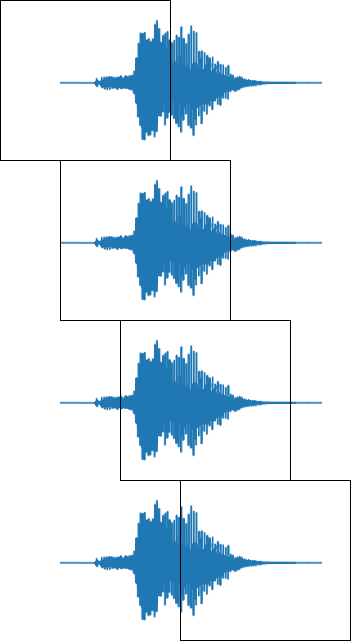
\includegraphics[width=0.4\linewidth]{Chapters/struktura_sustava/aktivacija_nn/timeline.png}
    \caption{Uzastopni vremenski okviri (prozori) \cite{flowchart}}
    \label{pic:timeline}
\end{figure}

Na slici \ref{pic:timeline} prikazani su uzastopni vremenski prozori nad ulaznim zvučnim signalom.
Na signalu je vidljiv vremenski odsječak u kojem je izgovorena naredba, a prije i poslije
izgovorene naredbe je tišina. U drugom i trećem prozoru očekuje se velika vjerojatnost da 
je prepoznata izgovorena naredba, dok se u prvom i četvrtom prozoru ne očekuje prepoznavanje
određene naredbe (u tim prozorima veću vjerojatnost imaju kategorije "nepoznato" ili "pozadina").
Upravo zbog prikazanog je potrebno što češće aktivirati mrežu i ne propustiti prepoznavanje naredbe. 
U slučaju da smo aktivirali mrežu rjeđe, ne bismo prepoznali naredbu (npr. prvi pa četvrti
prozor). 

No, takav pristup otvara mjesto drugom problemu. Ne želimo niti višestruko prepoznavanje
jednom izgovorene naredbe. Tu na scenu stupa podsustav za prepoznavanje i okidanje naredbi.